% Beamer slide template prepared by Tom Clark <tom.clark@op.ac.nz>
% Otago Polytechnic
% Dec 2012

\documentclass[10pt]{beamer}
\usetheme{Dunedin}
\usepackage{graphicx}
\usepackage{fancyvrb}

\newcommand\codeHighlight[1]{\textcolor[rgb]{1,0,0}{\textbf{#1}}}

\title{The Observer Pattern}

\author[IN608]{Intermediate Application Development}
\institute[Otago Polytechnic]{
  Otago Polytechnic \\
  Dunedin, New Zealand \\
  Kaiako: Tom Clark
}
\date{}
\begin{document}

%----------- titlepage ----------------------------------------------%
\begin{frame}[plain]
  \titlepage
\end{frame}

%----------- slide --------------------------------------------------%
\begin{frame}[fragile]
  \frametitle{Introduction}
  
  \vspace{5mm}
   ``Define a one-to-many dependency between objects so that when one object changes state,
   all its dependents are notified and updated automatically.'' \\
  (\emph{GoF})
  
  In this pattern we have one object, the \emph{Subject} that notifies other objects, 
  called \emph{Observers} whenever its state changes.
  
  \end{frame}

%----------- slide --------------------------------------------------%
\begin{frame}
  \frametitle{Examples}
  
  Suppose we have an object that represents some data, and multiple UI elements that need to update 
  when that data changes. In this case the data object is the Subject and the UI elements are observers.
  
    
\end{frame}



%----------- slide --------------------------------------------------%
\begin{frame}
  \frametitle{Structural Diagram} 
  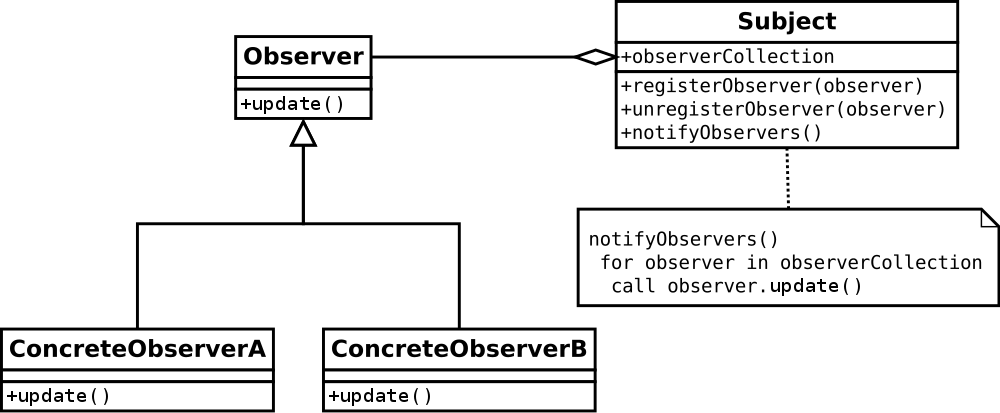
\includegraphics[width=8cm]{observer.png}
  \end{frame}
  

 
%----------- slide --------------------------------------------------%
\begin{frame}[fragile]
  \frametitle{Subject Class}

  \begin{verbatim}
  class Subject:
  
      def __init__(self):
          self._observers = set()
          
      def register(self, observer):
          self._observers.add(observer)
          
      def unregister(self, observer):
          self._observers.discard(observer)
          
      def notify(self):
          for o in self._observers:
              o.update(self)         
  \end{verbatim}
 \end{frame} 

%----------- slide --------------------------------------------------%
\begin{frame}[fragile]
  \frametitle{Observer Class}

  \begin{verbatim}
  class Observer:
      def update(subject):
          pass
      
  \end{verbatim}
 \end{frame} 


 %----------- slide --------------------------------------------------%
\begin{frame}
  \frametitle{Programming Activity}
  
  \begin{enumerate}
    \item Pull the course materials repo.
    \item Create a new branch, \texttt{13-practical} in your practicals repo.
    \item Add a subdirectory,  \texttt{13-practical} and copy \texttt{11-practical.ipynb} from the class materials into it.
    \item Open a shell, cd to this directory, and run \texttt{jupyter notebook} to open the notebook. Complete the first two questions.
    \item We will discuss results in 20ish minutes.
  \end{enumerate}      
\end{frame}

%----------- slide --------------------------------------------------%
\begin{frame}[fragile]
  \frametitle{A Pythonic Refinement}
  
  We can remove the requirement that Observers implement a method
  named exactly ``\texttt{update()}''.
  
  \begin{verbatim}
  class Subject:  
      def __init__(self):
          self._observers = {} # dictionary
          
      def register(self, observer, update_method):
          self._observers[observer] = update_method
          
      def unregister(self, observer):
          try:    
              del(self_observers[observer})
          except KeyError:
              pass
              
      def notify(self):
          for update in self._observers.values():
              update{self)
                      
  \end{verbatim} 
       
\end{frame} 

%----------- slide --------------------------------------------------%
\begin{frame}
  \frametitle{Publish-Subscribe Variation}
  
   It's also possible to take the decoupling a step further, with 
   what is sometimes called the Publish-Subscribe pattern. 
  
       
  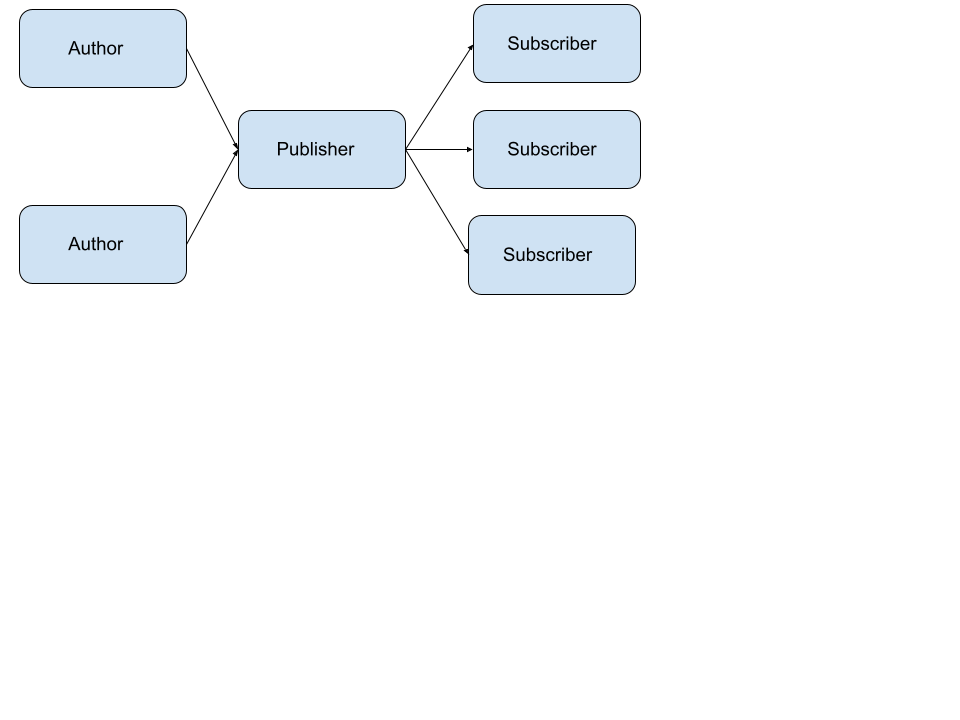
\includegraphics[width=8cm]{pub-sub.png}
       
\end{frame} 



\end{document}
